\section{Koši kriterijus}

\begin{note}
  Toliau tekste daroma prielaida, jog $f: A \to \RSET$ ir $a$ yra 
  aibės $A$ ribinis taškas.
\end{note}

\begin{prop}
  (Koši kriterijus) Funkcija $f$ turi baigtinę ribą taške $a$
  (taškas $a$ gali būti ir $\infty$) tada ir tik tada:
  \begin{equation}
    \forall \varepsilon (\varepsilon > 0), \exists U_{a} :
    | f(x') - f(x'') | < \varepsilon,
    \forall x', x'' (x',x'' \in U_{a} \cap A, x' \neq a, x'' \neq a)
    \label{kosi}
  \end{equation}

  \begin{proof}
    \hfill \\
    \begin{description}
      \item[Būtinumas] Tarkime, jog $\exists \lim _{x \to a} f(x)$ ir ji
        yra baigtinė. Reikia įrodyti \ref{kosi} teiginį.

        Pažymėkime:
        \begin{equation*}
          \lim _{x \to a} f(x) = b.
        \end{equation*}

        Tada pagal funkcijos ribos apibrėžimą (\ref{limfed}):
        \begin{equation*}
          \lim _{x \to a} f(x) = b \iff 
          \forall \varepsilon (\varepsilon > 0), \exists U_{a}:
          | f(x) - b | < \varepsilon, 
          \forall x (x \in U_{a} \cap A \setminus \{a\}).
        \end{equation*}

        Tada galime įvertinti:
        \begin{align*}
          | f(x') - f(x'') | &= | f(x') - b + b - f(x'') | \\
          &\leq \underbrace{| f(x') - b |}_{ < \varepsilon } +
          \underbrace{| f(x'') - b |}_{ < \varepsilon } \\
          &< 2 \varepsilon, \forall x',x'' 
          (x',x'' \in U_{a} \cap A \setminus \{a\}).
        \end{align*}

      \item[Pakankamumas] Tarkime, kad \ref{kosi} sąlyga teisinga. Reikia 
        įrodyti, kad $\exists \lim _{x \to a} f(x)$ ir kad ji yra baigtinė.

        Kadangi \ref{kosi} teisinga, tai:
        \begin{equation}
          \forall \varepsilon (\varepsilon > 0), \exists U_{a} :
          | f(x') - f(x'') | < \varepsilon, \forall x',x''
          (x',x'' \in U_{a} \cup A \setminus \{a\})
          \label{_kosi_01}
        \end{equation}

        Imame bet kokią seką $\left\{ x_{n} \right\}, x_{n} \to a$. Pagal
        sekos ribos apibrėžimą:
        \begin{equation}
          \forall U_{a}, \exists N : x_{n} \in U_{a}, \forall n (n > \NSET)
          \label{_kosi_02}
        \end{equation}

        Tada iš \ref{_kosi_01} ir \ref{_kosi_02} gauname:
        \begin{equation}
          | f(x_{n}) - f(x_{m}) | < \varepsilon : \forall n, m (n,m > N)
          \label{_kosi_03}
        \end{equation}

        Iš Koši kriterijaus skaičių sekoms ir \ref{_kosi_03} gauname, kad
        seka $\left\{ f(x_{n}) \right\}$ turi baigtinę ribą.

        Tam, kad pilnai būtų patenkintas \ref{limfs} funkcijos ribos 
        apibrėžimas, reikia, kad ir 
        $\left\{ x'_{n} \right\} x'_{n} \to a : \left\{ f(x'_{n}) \right\}$
        turėtų tą pačią ribą, kaip ir $\left\{ f(x_{n}) \right\}$, 
        kai $x_{n} \to a$.

        Sukonstruokime seką
        \begin{equation*}
          x_{1},x'_{1},x_{2},x'_{2},x_{3},x'_{3},\ldots
        \end{equation*}
        ir pažymėkime ją $\left\{ y_{n} \right\}$.

        Kadangi sekos $\left\{ y_{n} \right\}$ posekiai 
        $\left\{ x_{n} \right\}$ ir $\left\{ x'_{n} \right\}$, kurie pilnai 
        padengia visus jos narius, artėja į $a$, tai ir seka 
        $\left\{ y_{n} \right\}$ artėja į $a$.

        Iš Koši kriterijaus skaičių sekoms gauname, jog 
        $\left\{ f(y_{n}) \right\}$ turi baigtinę ribą. Iš skaičių sekos
        ribos apibrėžimo neprieštaringumo gauname, jog 
        $\left\{ f(y_{2n}) \right\} = \left\{ f(x'_{n}) \right\}$ ir
        $\left\{ f(y_{2n+1}) \right\} = \left\{ f(x_{n}) \right\}$ turi tą
        pačią ribą.

    \end{description}
  \end{proof}
\end{prop}

\section{Ribų skaičiavimo pavyzdžiai}

\begin{exmp}
  \label{lim_sinx_x}
  Įrodysime, kad:
  \begin{equation*}
    \lim _{x \to 0} \frac{\sin x}{x} = 1
  \end{equation*}

  \begin{proof}

    Nubrėžkime vienetinį apskritimą ($|OD| = |OB| = 1$). Iš 
    brėžinio (\ref{fig:sinx_x}) matome, jog:
    \begin{equation}
      S _{\triangle OBD} \leq S _{\text{išp.}OBD} \leq S _{\triangle OBC}
      \label{_sinx_x_01}
    \end{equation}

    \begin{figure}[h!]
      \begin{center}
        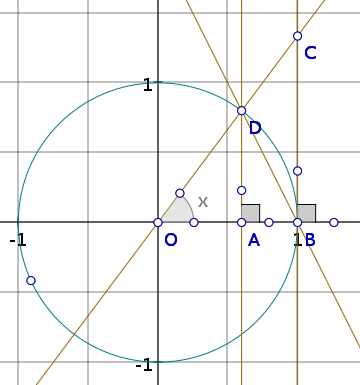
\includegraphics[]{images/sinx_x.png}
      \end{center}
      \caption{Brėžinys.}
      \label{fig:sinx_x}
    \end{figure}

    Apskaičiuokime trikampio $ODB$ plotą:
    \begin{align*}
      S _{\triangle OBD} &= \frac{ |AD| |OB| }{2} \\
      &= \frac{ |AD| }{2}, &\left\{ \text{ nes } |OB| = 1 \right\} \\
      &= \frac{ |OD| \sin x }{2}, 
      &\left\{ \text{ nes } \frac{ |AD| }{ |OD| } = \sin x \right\} \\
      &= \frac{ \sin x }{2}, &\left\{ \text{ nes } |OD| = 1 \right\}.
    \end{align*}

    Skritulio plotas lygus:
    \begin{equation*}
      S = \pi |OD|^2
    \end{equation*}

    Išpjovos $S_{\text{išp.}OBD}$ plotas sudaro $\frac{x}{2 \pi}$ viso 
    skritulio ploto:
    \begin{align*}
      S_{\text{išp.}OBD} &= S \frac{x}{2 \pi} \\
      &= \frac{\pi |OD|^2 x}{2 \pi} \\
      &= \frac{x}{2}
    \end{align*}

    Apskaičiuokime trikampio $OBC$ plotą:
    \begin{align*}
      S_{\triangle OBC} &= \frac{ |OB| |BC| }{2} \\
      &= \frac{ |OB| (|OB| \tg x)}{2}, 
        &\left\{ \text{ nes } \frac{|BC|}{|OB} = \tg x \right\} \\
      &= \frac{\tg x}{2} &\left\{ \text{ nes } |OB| = 1 \right\}
    \end{align*}

    Įsistatę išraiškas į \ref{_sinx_x_01} gauname:
    \begin{equation*}
      \frac{\sin x}{2} \leq \frac{x}{2} \leq \frac{\tg x}{2}
    \end{equation*}

    Pertvarkę gauname:
    \begin{align}
      \sin x \leq x & \text{ ir } \label{_sinx_x_02} \\
      x \leq \tg x. \label{_sinx_x_03}
    \end{align}

    Iš \ref{_sinx_x_02} gauname:
    \begin{equation}
      \frac{\sin x}{x} \leq 1 
      \label{_sinx_x_04}
    \end{equation}

    O iš \ref{_sinx_x_03}:
    \begin{align}
      x & \leq \tg x = \frac{\sin x}{\cos x} \\
      \cos x &\leq \frac{\sin x}{x}.
      \label{_sinx_x_05}
    \end{align}

    Iš \ref{_sinx_x_04} ir \ref{_sinx_x_05}:
    \begin{align}
      \cos x &\leq \frac{\sin x}{x} \leq 1 \\
      \cos x - 1 &\leq \frac{\sin x}{x} - 1 \leq 0 \\
      0 &\leq 1 - \frac{\sin x}{x} \leq 1 - \cos x
    \end{align}

    Pasinaudodami \ref{f_tri_kvsum} ir \ref{f_tri_dkcos} trigonometrinėmis
    tapatybėmis $1 - \cos x$ galime pertvarkyti:
    \begin{align}
      1 - \cos x &= \left( \cos^2 \frac{x}{2} + \sin^2 \frac{x}{2} \right) 
        - \left( \cos^2 \frac{x}{2} - \sin^2 \frac{x}{2} \right) \\
      &= 2 \sin^2 \frac{x}{2} \\
      &\leq 2 \left( \frac{x}{2} \right)^2 
        &\left\{ \text{Pasinaudojame \ref{_sinx_x_02} neligybe.} \right\} \\
      &= \frac{x^2}{2}.
    \end{align}

    Pagal trijų girtuoklių teoremą, kadangi:
    \begin{align*}
      \lim _{x \to 0^{+}} 0 &= 0 &\text{ ir } \\
      \lim _{x \to 0^{+}} \frac{x^2}{2} &= 0 &\text{ tai ir } \\
      \lim _{x \to 0^{+}} \left( 1 - \frac{\sin x}{x} \right) &= 0, 
        &\text{o tai reiškia, kad} \\
      \lim _{x \to 0^{+}} \frac{\sin x}{x} &= 1.
    \end{align*}

    Pažymėję $y = -x$, gauname:
    \begin{align*}
      \lim _{x \to 0^{-}} \frac{\sin x}{x} &=
      \lim _{x \to 0^{-}} \frac{-\sin x}{-x} \\
      &= \lim _{x \to 0^{-}} \frac{\sin(-x)}{-x} \\
      &= \lim _{y \to 0^{+}} \frac{\sin y}{y} = 1
    \end{align*}

    Kadangi egzistuoja riba iš dešinės ir iš kairės, ir jos sutampa, tai
    \begin{equation*}
      \lim _{x \to 0} \frac{\sin x}{x} = 1
    \end{equation*}

  \end{proof}

\end{exmp}

\begin{exmp}
  Įrodysime, kad:
  \begin{equation}
    \lim _{x \to 0} (1 + x)^{\frac{1}{x}} = e
    \label{_fx_e_01}
  \end{equation}

  \begin{proof}

    Iš pradžių įrodysime, kad funkcijos $f(x) = (1 + x)^{\frac{1}{x}}$ 
    riba iš dešinės taške $x = 0$ yra lygi $e$.

    Sakykime, $x_k > 0$ ir $x_k \to 0 (k \in \NSET)$. Pažymėkime $n_k$ 
    mažiausią natūrinį skaičių, didesnį už $\frac{1}{x_k}$, tai yra 
    \begin{equation*}
      n_{k} = min \left\{ n \in \NSET : n > \frac{1}{x_{k}} \right\}
    \end{equation*}
    Iš Archimedo principo žinome, kad toks skaičius visada egzistuoja.
    Dabar galime įvertinti $\frac{1}{x_k}$:
    \begin{equation*}
      n_k - 1 \leq \frac{1}{x_k} < n_k.
    \end{equation*}

    Atlikę trivialius pertvarkymus gauname $x_k$ įvertinimą:
    \begin{equation*}
      \frac{1}{n_{k}} < x_k \leq \frac{1}{n_{k} - 1}.
    \end{equation*}

    Akivaizdu, kad $(1 + x_{k})^\frac{1}{x_{k}}$ pagrindą ir laipsnį 
    pakeitę ne didesniais, gausime ne didesnį skaičių. Tai yra:
    \begin{equation}
      \left( 1 + \frac{1}{n_{k}} \right)^{n_{k} - 1}
      \leq (1 + x_{k})^\frac{1}{x_{k}}.
      \label{_fx_e_03}
    \end{equation}

    Taip pat pakeitę ne mažesniais gausime ne mažesnį skaičių:
    \begin{equation}
      (1 + x_{k})^{\frac{1}{x_{k}}} 
      \leq \left( 1 + \frac{1}{n_{k} - 1} \right)^{n_{k}}
      \label{_fx_e_04}
    \end{equation}

    Kairiąją \ref{_fx_e_03} nelygybės pusę galime pertvarkyti į 
    \begin{equation}
      \underbrace{\left( 1 + \frac{1}{n_{k}} \right)^{-1}}_{\to 1}
      \underbrace{\left( 1 + \frac{1}{n_{k}} \right)^{n_{k}}}_{\to e}
      \label{_fx_e_05}
    \end{equation}

    Dešiniąją \ref{_fx_e_04} nelygybės pusę galime pertvarkyti į
    \begin{equation}
      \underbrace{\left( 1 + \frac{1}{n_{k}-1} \right)^{n_{k}-1}}_{\to e}
      \underbrace{\left( 1 + \frac{1}{n_{k}-1} \right)^{1}}_{\to 1}
      \label{_fx_e_06}
    \end{equation}

    Kadangi skaičių $y_{n} = (1 + \frac{1}{n})^n$ seka, kai 
    $n \to +\infty$, turi ribą $e$, tai ir seka $y_{n_{k}}$, kuri
    gali skirtis nuo sekos $y_{n}$ posekio tik narių tvarka turi 
    tą pačią ribą $e$. Taigi \ref{_fx_e_05} ir \ref{_fx_e_06} 
    konverguoja į skaičių $e$. Todėl, pagal dviejų policininkų
    principą, ir seka $(1 + x_{k})^{\frac{1}{x_{k}}}$ konverguoja į
    $e$. Pagal funkcijos ribos apibrėžimą sekoms (\ref{limfs})
    gauname:
    \begin{equation}
      \lim _{x \to 0^{+}} (1 + x)^{\frac{1}{x}} = e.
      \label{_fx_e_07}
    \end{equation}

    Dabar įrodysime, kad ir 
    $\lim _{x \to 0^{-}} (1 + x)^{\frac{1}{x}} = e$. Sakykime, kad
    $-1 < x < 0$ ir pažymėkime $y = -x$. Tada
    \begin{align*}
      \lim _{x \to 0^{-}} (1 + x)^{\frac{1}{x}} 
      &= \lim _{y \to 0^{+}} (1 - y)^{-\frac{1}{y}} \\
      &= \lim _{y \to 0^{+}} 
        \left( \frac{1}{1 - y} \right)^{\frac{1}{y}} \\
      &= \lim _{y \to 0^{+}} 
        \left( 1 + \frac{1}{1 - y} - 1 \right)^{\frac{1}{y}} \\
      &= \lim _{y \to 0^{+}} 
        \left( 1 + \frac{y}{1 - y} \right)^{\frac{1}{y}} \\
      &= \lim _{y \to 0^{+}} 
        \left( 1 + \frac{y}{1 - y} \right)^{\frac{1}{y} - 1}
        \left( 1 + \frac{y}{1 - y} \right)^{1} \\
      &= \lim _{y \to 0^{+}} 
        \underbrace{
          \left( 1 + \frac{y}{1 - y} \right)^{\frac{1 - y}{y}}}_{\to e}
        \underbrace{
          \left( 1 + \frac{y}{1 - y} \right)^{1}}_{\to 1} \\
      &= e.
    \end{align*}

  \end{proof}
\end{exmp}
